\chapter{The Critical Section Problem}

\section{Introduction to Concurrency}

Concurrency refers to the execution of multiple tasks during overlapping time periods. Modern operating systems support concurrency through processes, threads, multicore processors, and distributed systems.

Concurrency improves:

\begin{itemize}
\item CPU utilization
\item Responsiveness
\item Throughput
\item Scalability
\end{itemize}

However, concurrency introduces synchronization challenges when multiple execution units access shared resources.

\subsection{Concurrent Execution}

\begin{figure}[H]
\centering
\begin{tikzpicture}

\draw[->] (0,0) -- (10,0);
\node at (10.5,0) {Time};

\draw (1,2) -- (3,2);
\draw (4,2) -- (6,2);
\draw (7,2) -- (9,2);

\draw (2,1) -- (5,1);
\draw (6,1) -- (8,1);

\node[left] at (0,2) {Thread A};
\node[left] at (0,1) {Thread B};

\end{tikzpicture}
\caption{Concurrent Execution Timeline}
\end{figure}

\section{Shared Resources}

A shared resource is any resource accessible by multiple threads or processes.

Examples include:

\begin{itemize}
\item Shared variables
\item Memory regions
\item Files
\item Databases
\item Printers
\item Network sockets
\end{itemize}

\subsection{Shared Counter Example}

\begin{lstlisting}[language=C++,style=interviewcode]
int counter = 0;

Thread 1:
counter++;

Thread 2:
counter++;
\end{lstlisting}

At first glance the final value appears to be 2.

However concurrent execution can produce unexpected results.

\section{Race Conditions}

A race condition occurs when the output depends on the timing or order of execution of concurrent operations.

\subsection{Example}

Assume:

\[
counter = 5
\]

Two threads execute:

\begin{lstlisting}[language=C++,style=interviewcode]
counter++;
\end{lstlisting}

Internally:

\begin{enumerate}
\item Read counter
\item Increment value
\item Write back
\end{enumerate}

\subsection{Execution Timeline}

\begin{longtable}{|c|c|c|}
\hline
Step & Thread 1 & Thread 2 \\
\hline
1 & Read 5 & \\
\hline
2 & & Read 5 \\
\hline
3 & Compute 6 & \\
\hline
4 & & Compute 6 \\
\hline
5 & Write 6 & \\
\hline
6 & & Write 6 \\
\hline
\end{longtable}

Final value:

\[
6
\]

Expected value:

\[
7
\]

This is a race condition.

\section{Critical Sections}

A critical section is a code segment that accesses shared resources.

Only one thread should execute a critical section at a time.

\subsection{Structure}

\begin{figure}[H]
\centering
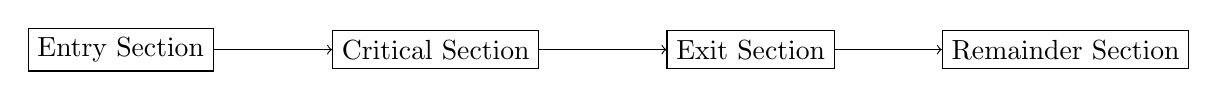
\begin{tikzpicture}

\node[draw] (entry) at (0,0) {Entry Section};

\node[draw] (critical) at (4,0) {Critical Section};

\node[draw] (exit) at (8,0) {Exit Section};

\node[draw] (remainder) at (12,0) {Remainder Section};

\draw[->] (entry)--(critical);
\draw[->] (critical)--(exit);
\draw[->] (exit)--(remainder);

\end{tikzpicture}
\caption{Critical Section Structure}
\end{figure}

\section{The Critical Section Problem}

The critical section problem asks:

\textit{How can multiple processes or threads safely share resources while preventing race conditions?}

The solution must satisfy three fundamental requirements.

\section{Requirements for a Correct Solution}

\subsection{Mutual Exclusion}

At most one process can execute inside the critical section at any time.

\begin{center}
Allowed:
\end{center}

\[
P_1 \rightarrow CS
\]

\[
P_2 \rightarrow Waiting
\]

\subsection{Progress}

If no process is in the critical section and some wish to enter, selection should not be postponed indefinitely.

\subsection{Bounded Waiting}

A process should not wait forever after requesting access.

There must exist an upper bound on waiting time.

\section{Software-Based Solutions}

Before hardware synchronization primitives existed, software algorithms attempted to solve the critical section problem.

Examples:

\begin{itemize}
\item Peterson's Algorithm
\item Bakery Algorithm
\end{itemize}

\section{Peterson's Algorithm}

Peterson's Algorithm solves the critical section problem for two processes.

\subsection{Shared Variables}

\begin{lstlisting}[language=C++,style=interviewcode]
bool flag[2];
int turn;
\end{lstlisting}

\subsection{Process i}

\begin{lstlisting}[language=C++,style=interviewcode]
flag[i] = true;
turn = j;

while(flag[j] && turn == j);

critical_section();

flag[i] = false;
\end{lstlisting}

\subsection{Working Principle}

\begin{enumerate}
\item Process announces intent.
\item Gives turn to other process.
\item Waits if other process also wants entry.
\item Enters critical section safely.
\end{enumerate}

\subsection{State Diagram}

\begin{figure}[H]
\centering
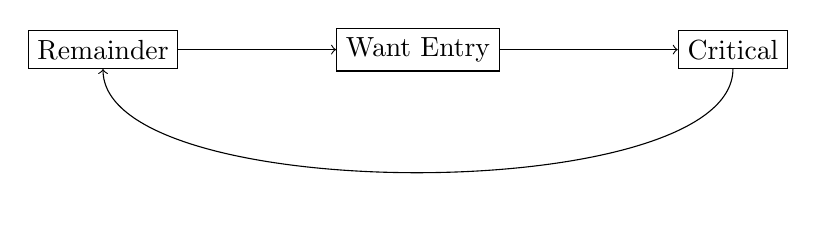
\begin{tikzpicture}

\node[draw] (rem) at (0,0) {Remainder};

\node[draw] (want) at (4,0) {Want Entry};

\node[draw] (crit) at (8,0) {Critical};

\draw[->] (rem)--(want);
\draw[->] (want)--(crit);
\draw[->] (crit) .. controls +(0,-2) and +(0,-2) .. (rem);

\end{tikzpicture}
\caption{Peterson's Algorithm States}
\end{figure}

\subsection{Interview Note}

Peterson's algorithm is important theoretically but rarely used in production systems because modern CPUs reorder memory operations.

\section{Bakery Algorithm}

Proposed by Leslie Lamport.

Inspired by customers taking numbered tickets in a bakery.

\subsection{Idea}

\begin{enumerate}
\item Each process takes a number.
\item Smallest ticket enters first.
\item Ties broken using process ID.
\end{enumerate}

\subsection{Example}

\begin{longtable}{|c|c|}
\hline
Process & Ticket \\
\hline
P1 & 5 \\
\hline
P2 & 2 \\
\hline
P3 & 7 \\
\hline
\end{longtable}

Execution order:

\[
P2 \rightarrow P1 \rightarrow P3
\]

\subsection{Advantages}

\begin{itemize}
\item Supports multiple processes
\item Guarantees fairness
\item Satisfies bounded waiting
\end{itemize}

\section{Hardware Support for Synchronization}

Software-only solutions are difficult to implement correctly on modern hardware.

Processors provide atomic instructions.

Benefits:

\begin{itemize}
\item Faster synchronization
\item Simpler implementation
\item Better scalability
\end{itemize}

\section{Atomic Operations}

An atomic operation executes completely or not at all.

No interruption occurs during execution.

Examples:

\begin{itemize}
\item Test-and-Set
\item Compare-and-Swap
\item Exchange
\item Atomic Increment
\end{itemize}

\subsection{Atomicity Illustration}

\begin{figure}[H]
\centering
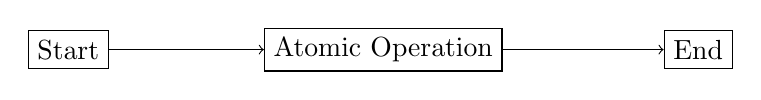
\begin{tikzpicture}

\node[draw] (start) at (0,0) {Start};

\node[draw] (atomic) at (4,0) {Atomic Operation};

\node[draw] (end) at (8,0) {End};

\draw[->] (start)--(atomic);
\draw[->] (atomic)--(end);

\end{tikzpicture}
\caption{Atomic Execution}
\end{figure}

\section{Test-and-Set Instruction}

Test-and-Set atomically reads and sets a memory location.

\subsection{Pseudo Code}

\begin{lstlisting}[language=C++,style=interviewcode]
bool TestAndSet(bool *lock)
{
    bool old = *lock;
    *lock = true;
    return old;
}
\end{lstlisting}

\subsection{Spinlock Example}

\begin{lstlisting}[language=C++,style=interviewcode]
while(TestAndSet(&lock));

critical_section();

lock = false;
\end{lstlisting}

\section{Compare-and-Swap (CAS)}

CAS compares memory content with an expected value.

If equal, replacement occurs atomically.

\subsection{Pseudo Code}

\begin{lstlisting}[language=C++,style=interviewcode]
CAS(address, expected, newValue)
\end{lstlisting}

\subsection{Example}

\begin{lstlisting}[language=C++,style=interviewcode]
int expected = 10;

CAS(&x, expected, 20);
\end{lstlisting}

If:

\[
x = 10
\]

then:

\[
x = 20
\]

Otherwise no change occurs.

\section{Exchange Instruction}

Exchange atomically swaps values.

\subsection{Pseudo Code}

\begin{lstlisting}[language=C++,style=interviewcode]
Exchange(&a, &b);
\end{lstlisting}

\subsection{Use Cases}

\begin{itemize}
\item Locks
\item Spinlocks
\item Atomic ownership transfer
\end{itemize}

\section{Spinlocks}

A spinlock repeatedly checks a lock variable.

\subsection{Operation}

\begin{enumerate}
\item Attempt lock acquisition.
\item If unavailable, spin.
\item Acquire lock.
\item Execute critical section.
\item Release lock.
\end{enumerate}

\subsection{Visualization}

\begin{figure}[H]
\centering
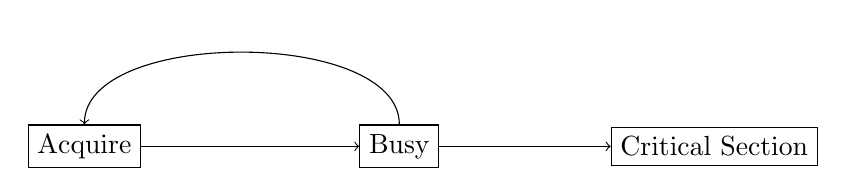
\begin{tikzpicture}

\node[draw] (try) at (0,0) {Acquire};

\node[draw] (busy) at (4,0) {Busy};

\node[draw] (cs) at (8,0) {Critical Section};

\draw[->] (try)--(busy);

\draw[->] (busy) .. controls +(0,1.5) and +(0,1.5) .. (try);

\draw[->] (busy)--(cs);

\end{tikzpicture}
\caption{Spinlock Behavior}
\end{figure}

\subsection{Advantages}

\begin{itemize}
\item Low overhead
\item Efficient for short waits
\end{itemize}

\subsection{Disadvantages}

\begin{itemize}
\item CPU wastage
\item Poor for long waits
\end{itemize}

\section{Modern CPU Challenges}

Modern processors introduce complexities:

\begin{itemize}
\item Out-of-order execution
\item Multiple cache levels
\item Memory reordering
\item Store buffers
\item Multiple cores
\end{itemize}

Traditional algorithms may fail without memory barriers.

\section{Memory Reordering Basics}

Processors may reorder instructions to improve performance.

\subsection{Example}

Program order:

\begin{lstlisting}[language=C++,style=interviewcode]
x = 1;
flag = true;
\end{lstlisting}

Observed order:

\begin{lstlisting}[language=C++,style=interviewcode]
flag = true;
x = 1;
\end{lstlisting}

Another CPU may observe the reordered version.

\subsection{Memory Illustration}

\begin{figure}[H]
\centering
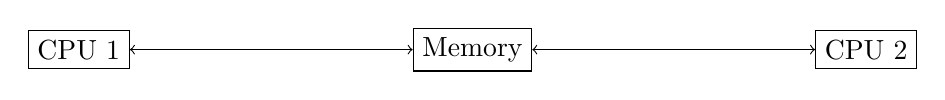
\begin{tikzpicture}

\node[draw] (cpu1) at (0,0) {CPU 1};

\node[draw] (mem) at (5,0) {Memory};

\node[draw] (cpu2) at (10,0) {CPU 2};

\draw[<->] (cpu1)--(mem);
\draw[<->] (cpu2)--(mem);

\end{tikzpicture}
\caption{Shared Memory Visibility Challenges}
\end{figure}

\section{Real-World Race Condition Examples}

\subsection{Bank Account Update}

\begin{lstlisting}[language=C++,style=interviewcode]
balance = balance - 100;
\end{lstlisting}

Simultaneous withdrawals may corrupt the balance.

\subsection{Inventory Management}

Two orders simultaneously decrement stock.

Result:

Negative inventory.

\subsection{Ticket Booking}

Two users purchase the last seat concurrently.

Result:

Overbooking.

\subsection{Web Counter}

\begin{lstlisting}[language=C++,style=interviewcode]
visitors++;
\end{lstlisting}

Concurrent updates lose increments.

\section{Interview Explanations}

\subsection{Why is the Critical Section Problem Important?}

Almost every concurrent application accesses shared resources.

Without synchronization:

\begin{itemize}
\item Data corruption occurs.
\item Results become nondeterministic.
\item Bugs become difficult to reproduce.
\end{itemize}

\subsection{Why Isn't Peterson's Algorithm Used in Practice?}

Modern hardware reorders memory operations.

The algorithm assumes strict memory ordering.

\subsection{Why Is CAS Popular?}

CAS is lock-free and supported by modern CPUs.

Many concurrent data structures use CAS internally.

\subsection{Spinlock vs Mutex}

Spinlocks waste CPU cycles while waiting.

Mutexes put threads to sleep.

Spinlocks are preferred only for short critical sections.

\section{Common Mistakes}

\begin{itemize}
\item Assuming increment operations are atomic.
\item Forgetting memory visibility issues.
\item Holding locks too long.
\item Using spinlocks for long waits.
\item Ignoring fairness requirements.
\item Accessing shared data without synchronization.
\item Assuming multicore execution is deterministic.
\end{itemize}

\section{Key Takeaways}

\begin{keytakeaways}
Concurrency introduces race conditions when multiple execution units access shared resources. The critical section problem seeks safe access to shared data while satisfying mutual exclusion, progress, and bounded waiting. Peterson's and Bakery algorithms provide theoretical software solutions. Modern systems rely on atomic hardware instructions such as Test-and-Set, Compare-and-Swap, and Exchange. Spinlocks provide lightweight synchronization but must be used carefully. Modern CPUs introduce memory reordering challenges that require additional synchronization guarantees.
\end{keytakeaways}

\section{Interview Questions with Answers}

\begin{enumerate}
\item What is a race condition?\\
A bug caused by concurrent unsynchronized access to shared data.

\item What is a critical section?\\
Code accessing shared resources.

\item What is mutual exclusion?\\
Only one thread can enter the critical section at a time.

\item What is progress?\\
Eligible threads should not be indefinitely postponed.

\item What is bounded waiting?\\
A waiting thread must eventually gain access.

\item What is Peterson's algorithm?\\
A software solution for two-process synchronization.

\item What are Peterson's shared variables?\\
flag[] and turn.

\item What is Lamport's Bakery algorithm?\\
A ticket-based synchronization algorithm.

\item What is an atomic operation?\\
An indivisible operation.

\item What is Test-and-Set?\\
An atomic instruction used for locking.

\item What is CAS?\\
Compare-and-Swap atomic primitive.

\item What is Exchange?\\
Atomic swapping of values.

\item What is a spinlock?\\
A lock that repeatedly checks availability.

\item Why are spinlocks expensive?\\
They consume CPU while waiting.

\item Why are locks needed?\\
To prevent race conditions.

\item What causes memory reordering?\\
CPU performance optimizations.

\item Why can increments be unsafe?\\
They involve multiple machine operations.

\item What is lock-free programming?\\
Concurrency using atomic primitives instead of locks.

\item Why is fairness important?\\
To avoid starvation.

\item What is starvation?\\
Indefinite waiting for resource access.
\end{enumerate}

\section{MCQs with Answers}

\begin{enumerate}
\item A race condition occurs due to:
\begin{enumerate}[label=(\alph*)]
\item Paging
\item Shared access
\item Segmentation
\item Swapping
\end{enumerate}
Answer: (b)

\item Critical section accesses:
\begin{enumerate}[label=(\alph*)]
\item Private data
\item Shared data
\item Cache only
\item Stack only
\end{enumerate}
Answer: (b)

\item Mutual exclusion allows:
\begin{enumerate}[label=(\alph*)]
\item One process inside
\item Many processes inside
\item No process inside
\item Infinite processes
\end{enumerate}
Answer: (a)

\item Peterson's algorithm supports:
\begin{enumerate}[label=(\alph*)]
\item Two processes
\item Three processes
\item Four processes
\item Unlimited processes
\end{enumerate}
Answer: (a)

\item Bakery algorithm was proposed by:
\begin{enumerate}[label=(\alph*)]
\item Dijkstra
\item Lamport
\item Knuth
\item Hoare
\end{enumerate}
Answer: (b)

\item CAS stands for:
\begin{enumerate}[label=(\alph*)]
\item Compare-and-Swap
\item Check-and-Store
\item Compare-and-Store
\item Check-and-Swap
\end{enumerate}
Answer: (a)

\item Test-and-Set is:
\begin{enumerate}[label=(\alph*)]
\item Atomic
\item Blocking
\item Distributed
\item Sequential
\end{enumerate}
Answer: (a)

\item Spinlocks are useful for:
\begin{enumerate}[label=(\alph*)]
\item Long waits
\item Short waits
\item Disk access
\item Paging
\end{enumerate}
Answer: (b)

\item Bounded waiting prevents:
\begin{enumerate}[label=(\alph*)]
\item Deadlock
\item Starvation
\item Paging
\item Swapping
\end{enumerate}
Answer: (b)

\item Progress ensures:
\begin{enumerate}[label=(\alph*)]
\item Eventual decision
\item Infinite wait
\item Memory safety
\item Cache hit
\end{enumerate}
Answer: (a)

\item Exchange instruction:
\begin{enumerate}[label=(\alph*)]
\item Swaps values atomically
\item Creates thread
\item Deletes thread
\item Allocates memory
\end{enumerate}
Answer: (a)

\item Modern CPUs may:
\begin{enumerate}[label=(\alph*)]
\item Reorder memory operations
\item Remove memory
\item Disable caches
\item Disable registers
\end{enumerate}
Answer: (a)

\item Shared bank account updates require:
\begin{enumerate}[label=(\alph*)]
\item Synchronization
\item Paging
\item DMA
\item Segmentation
\end{enumerate}
Answer: (a)

\item Starvation means:
\begin{enumerate}[label=(\alph*)]
\item Infinite waiting
\item Memory leak
\item CPU crash
\item Cache miss
\end{enumerate}
Answer: (a)

\item Lock-free structures commonly use:
\begin{enumerate}[label=(\alph*)]
\item CAS
\item FIFO
\item DMA
\item MMU
\end{enumerate}
Answer: (a)

\item Peterson's algorithm uses:
\begin{enumerate}[label=(\alph*)]
\item turn variable
\item semaphore
\item mutex
\item queue
\end{enumerate}
Answer: (a)

\item Increment operation is:
\begin{enumerate}[label=(\alph*)]
\item Always atomic
\item Usually multiple steps
\item Kernel only
\item Single-core only
\end{enumerate}
Answer: (b)

\item Spinlocks waste:
\begin{enumerate}[label=(\alph*)]
\item CPU cycles
\item RAM
\item Disk
\item Network
\end{enumerate}
Answer: (a)

\item A synchronization primitive is:
\begin{enumerate}[label=(\alph*)]
\item CAS
\item Cache
\item DMA
\item PCB
\end{enumerate}
Answer: (a)

\item Critical section solutions require:
\begin{enumerate}[label=(\alph*)]
\item Mutual exclusion
\item Progress
\item Bounded waiting
\item All of the above
\end{enumerate}
Answer: (d)
\end{enumerate}

\section{Revision Notes}

\begin{revisionnotes}
\item Concurrency introduces race conditions.
\item Shared resources require synchronization.
\item Critical sections access shared data.
\item Mutual exclusion permits one thread at a time.
\item Progress prevents indefinite postponement.
\item Bounded waiting prevents starvation.
\item Peterson's algorithm works for two processes.
\item Bakery algorithm uses ticket ordering.
\item Atomic operations execute indivisibly.
\item Test-and-Set enables lock implementation.
\item CAS powers many lock-free algorithms.
\item Exchange atomically swaps values.
\item Spinlocks actively wait.
\item Modern CPUs reorder memory operations.
\item Memory visibility is critical in multicore systems.
\end{revisionnotes}

\section{Cheat Sheet}

\begin{longtable}{|p{5cm}|p{8cm}|}
\hline
Concept & Summary \\
\hline
Race Condition & Concurrent unsynchronized access \\
\hline
Critical Section & Shared resource access code \\
\hline
Mutual Exclusion & One thread inside at a time \\
\hline
Progress & No unnecessary postponement \\
\hline
Bounded Waiting & No starvation \\
\hline
Peterson's Algorithm & Two-process software solution \\
\hline
Bakery Algorithm & Ticket-based fairness \\
\hline
Atomic Operation & Indivisible execution \\
\hline
Test-and-Set & Atomic lock primitive \\
\hline
CAS & Compare-and-Swap \\
\hline
Exchange & Atomic value swap \\
\hline
Spinlock & Busy-wait lock \\
\hline
Memory Reordering & CPU optimization affecting visibility \\
\hline
Starvation & Infinite waiting \\
\hline
Lock-Free Programming & Uses atomic primitives instead of locks \\
\hline
\end{longtable}